\section*{Výsledky měření}
Nejprve jsme provedli energetickou kalibraci. Použili jsme tři známé peaky z gamma spektra $^{241}$Am: \SI{13.9}{\keV}, \SI{26.3}{\keV} a \SI{59.5}{\keV}. Další známý peak \SI{17.8}{\keV} jsme s novou kalibrací změřili na \SI{17.53}{\keV}, což nám dává představu o nejistotě měření energie.

Měřili jsme rentgenové spektrum celkem 7 čistých prvků a 2 dvouprvkových slitin. V tabulce \ref{t:merenivzorky} jsou uvedené naměřené energie pozorovaných přechodů a jejich výtěžek. Relativní chyba výtěžku je stejná jako \emph{net area}. Prvky jsme identifikovali podle přiložené tabulky energií charakteristického rentgenového záření. $E_t$ je tabelovaná energie přechodu \cite{energie}, uvádíme vždy přechod s posledním číslem 1 ve Siegbahnově notaci (K$\upalpha_1$, K$\upbeta_1$, L$\upalpha_1$, L$\upbeta_1$).

U Cu jsme naměřili pouze jeden peak mezi K$\upalpha$ a K$\upbeta$, což odpovídá tomu, že jsou blízké a nedokážeme rozlišit. U všech ostatních prvků kromě Pb se nám podařilo rozlišit dva peaky, a to K$\upalpha$ a K$\upbeta$. U Pb jsme pozorovali pouze L$\upalpha$ a L$\upbeta$.

\begin{tabulka}[htbp]
\centering
\begin{tabular}{c|ccccc|cc}
vzorek & $E$ (\si{\keV}) & FWHM (\si{\keV}) & net area & výtěžek (cps) & přechod & prvek & $E_t$ (\si{\eV})\\ \hline\hline

1 & 8,17 & 1,16 & \num{24205(251)} & \num{30,3(3)} & K$\upalpha$ a K$\upbeta$ & $_{29}$Cu & 8047 a 8905\\  \hline
\multirow{2}{*}{2} & 25,25 & 1,10 & \num{66467(331)} & \num{90,8(5)} & K$\upalpha$ & \multirow{2}{*}{$_{50}$Sn} & \num{25271}\\
 & 28,58 & 1,08 & \num{14171(190)} & \num{19,4(3)} & K$\upbeta$ &  & \num{28486}\\ \hline
\multirow{2}{*}{3} & 20,24 & 1,04 & \num{15116(171)} & \num{57,7(7)} & K$\upalpha$ & \multirow{2}{*}{$_{45}$Rh} & \num{20216}\\ 
 & 22,84 & 0,96 & \num{3120(103)} & 10,9(4) & K$\upbeta$ & & \num{22724}\\ \hline
\multirow{2}{*}{4} & 10,61 & 0,83 & \num{3556(112)} & 14,5(5) & L$\upalpha$ & \multirow{2}{*}{$_{82}$Pb} & \num{10552}\\ 
 & 12,67 & 0,90 & \num{3823(123)} & 15,6(5) & L$\upbeta$ & & \num{12613}\\ \hline
\multirow{2}{*}{11} & 23,16 & 1,02 & \num{17017(178)} & 83,4(9) & K$\upalpha$ & \multirow{2}{*}{$_{48}$Cd} & \num{23174}\\ 
 & 26,18 & 1,15 & \num{4489(111)} & 22,0(6) & K$\upbeta$ & & \num{26095}\\ \hline
\multirow{2}{*}{6} & 15,81 & 0,85 & \num{18116(249)} & 36,9(5) & K$\upalpha$ & \multirow{2}{*}{$_{40}$Zr} & \num{15775}\\
 & 17,67 & 0,62 & \num{1639(126)} & 3,3(3) & K$\upbeta$ &  & \num{17666}\\ \hline
\multirow{2}{*}{9} & 17,49 & 1,07 & \num{35230(274)} & 70,9(6) & K$\upalpha$ & \multirow{2}{*}{$_{42}$Mo} & \num{17479}\\ 
 & 19,70 & 0,8 & \num{3881(143)} & 7,8(3) & K$\upbeta$ &  & \num{19603}\\ \hline\hline
\multirow{3}{*}{5} & 8,43 & 1,28 & \num{3716(147)} & 5,5(2) & K$\upalpha$ a K$\upbeta$ & $_{29}$Cu & 8048 a 8907 \\
 & 22,15 & 1,02 & \num{23575(246)} & 34,7(4) & K$\upalpha$ & \multirow{2}{*}{$_{47}$Ag} & \num{22163}\\
 & 25,03 & 1,03 & \num{7557(161)} & 11,2(3) & K$\upbeta$ & & \num{24942}\\ \hline
\multirow{4}{*}{13} & 10,58 & 1,03 & \num{5293(129)} & 13,6(4) & L$\upalpha$ & \multirow{2}{*}{$_{82}$Pb} & \num{10552} \\ 
 & 12,71 & 0,91 & \num{4834(148)} & 12,5(4) & L$\upbeta$ &  & \num{12613}\\
 & 25,26 & 1,08 & \num{11483(158)} & 29,6(4) & K$\upalpha$ & \multirow{2}{*}{$_{50}$Sn} & \num{25271}\\
 & 28,60 & 1,12 & \num{2958(94)} & 7,6(3) & K$\upbeta$ &  & \num{28486}\\
\end{tabular}
\caption{Naměřené energetické přechody. V první části tabulky jsou čisté prvky, pod druhou tlustou čárou jsou slitiny.}
\label{t:merenivzorky}
\end{tabulka}

Graf závislosti výtěžku na protonovém čísle pro přechod K$\upalpha$ je v grafu \ref{g:vytezek}. Zahrnuli jsme i Cu, protože peak je mnohem blíže energii přechodu K$\upalpha$ než K$\upbeta$, což naznačuje, že se v celkovém výtěžku uplatňuje převážně. To se potvrdilo i u ostatních prvků, K$\upalpha$ je vždy několikanásobně silnější než K$\upbeta$.
Nemáme žádný teoretický předpoklad na tvar této závislosti, proto jsme jej proložili polynomy prvního a druhého stupně
\begin{equation}
v_1(Z)=(-60+2,9Z)\text{cps} \,,
\end{equation}
\begin{equation}
v_2(Z)=(139-7,6Z+0,13Z^2)\text{cps} \,.
\end{equation}

Oba fity se shodují ve výtěžku pro Ag přibližně \SI{75}{cps} a tuto hodnotu použijeme pro výpočet zastoupení prvků ve slitinách.
Podle \eqref{e:konc} jsme určili podíly prvků ve slitině číslo 5
\begin{equation}
w_{Cu}^5=\SI{28(5)}{\percent} \,,\qquad \qquad w_{Ag}^5=\SI{72(5)}{\percent}
\end{equation}
a ve slitině číslo 13
\begin{equation}
w_{Pb}^{13}=\SI{74(5)}{\percent} \,,\qquad \qquad w_{Sn}^{13}=\SI{26(5)}{\percent} \,.
\end{equation}

\begin{graph}[htbp] 
\centering
% GNUPLOT: LaTeX picture with Postscript
\begingroup
  \makeatletter
  \providecommand\color[2][]{%
    \GenericError{(gnuplot) \space\space\space\@spaces}{%
      Package color not loaded in conjunction with
      terminal option `colourtext'%
    }{See the gnuplot documentation for explanation.%
    }{Either use 'blacktext' in gnuplot or load the package
      color.sty in LaTeX.}%
    \renewcommand\color[2][]{}%
  }%
  \providecommand\includegraphics[2][]{%
    \GenericError{(gnuplot) \space\space\space\@spaces}{%
      Package graphicx or graphics not loaded%
    }{See the gnuplot documentation for explanation.%
    }{The gnuplot epslatex terminal needs graphicx.sty or graphics.sty.}%
    \renewcommand\includegraphics[2][]{}%
  }%
  \providecommand\rotatebox[2]{#2}%
  \@ifundefined{ifGPcolor}{%
    \newif\ifGPcolor
    \GPcolorfalse
  }{}%
  \@ifundefined{ifGPblacktext}{%
    \newif\ifGPblacktext
    \GPblacktexttrue
  }{}%
  % define a \g@addto@macro without @ in the name:
  \let\gplgaddtomacro\g@addto@macro
  % define empty templates for all commands taking text:
  \gdef\gplbacktext{}%
  \gdef\gplfronttext{}%
  \makeatother
  \ifGPblacktext
    % no textcolor at all
    \def\colorrgb#1{}%
    \def\colorgray#1{}%
  \else
    % gray or color?
    \ifGPcolor
      \def\colorrgb#1{\color[rgb]{#1}}%
      \def\colorgray#1{\color[gray]{#1}}%
      \expandafter\def\csname LTw\endcsname{\color{white}}%
      \expandafter\def\csname LTb\endcsname{\color{black}}%
      \expandafter\def\csname LTa\endcsname{\color{black}}%
      \expandafter\def\csname LT0\endcsname{\color[rgb]{1,0,0}}%
      \expandafter\def\csname LT1\endcsname{\color[rgb]{0,1,0}}%
      \expandafter\def\csname LT2\endcsname{\color[rgb]{0,0,1}}%
      \expandafter\def\csname LT3\endcsname{\color[rgb]{1,0,1}}%
      \expandafter\def\csname LT4\endcsname{\color[rgb]{0,1,1}}%
      \expandafter\def\csname LT5\endcsname{\color[rgb]{1,1,0}}%
      \expandafter\def\csname LT6\endcsname{\color[rgb]{0,0,0}}%
      \expandafter\def\csname LT7\endcsname{\color[rgb]{1,0.3,0}}%
      \expandafter\def\csname LT8\endcsname{\color[rgb]{0.5,0.5,0.5}}%
    \else
      % gray
      \def\colorrgb#1{\color{black}}%
      \def\colorgray#1{\color[gray]{#1}}%
      \expandafter\def\csname LTw\endcsname{\color{white}}%
      \expandafter\def\csname LTb\endcsname{\color{black}}%
      \expandafter\def\csname LTa\endcsname{\color{black}}%
      \expandafter\def\csname LT0\endcsname{\color{black}}%
      \expandafter\def\csname LT1\endcsname{\color{black}}%
      \expandafter\def\csname LT2\endcsname{\color{black}}%
      \expandafter\def\csname LT3\endcsname{\color{black}}%
      \expandafter\def\csname LT4\endcsname{\color{black}}%
      \expandafter\def\csname LT5\endcsname{\color{black}}%
      \expandafter\def\csname LT6\endcsname{\color{black}}%
      \expandafter\def\csname LT7\endcsname{\color{black}}%
      \expandafter\def\csname LT8\endcsname{\color{black}}%
    \fi
  \fi
  \setlength{\unitlength}{0.0500bp}%
  \begin{picture}(10204.00,6802.00)%
    \gplgaddtomacro\gplbacktext{%
      \csname LTb\endcsname%
      \put(946,704){\makebox(0,0)[r]{\strut{} 0}}%
      \csname LTb\endcsname%
      \put(946,1871){\makebox(0,0)[r]{\strut{} 20}}%
      \csname LTb\endcsname%
      \put(946,3037){\makebox(0,0)[r]{\strut{} 40}}%
      \csname LTb\endcsname%
      \put(946,4204){\makebox(0,0)[r]{\strut{} 60}}%
      \csname LTb\endcsname%
      \put(946,5370){\makebox(0,0)[r]{\strut{} 80}}%
      \csname LTb\endcsname%
      \put(946,6537){\makebox(0,0)[r]{\strut{} 100}}%
      \csname LTb\endcsname%
      \put(1078,484){\makebox(0,0){\strut{} 20}}%
      \csname LTb\endcsname%
      \put(2169,484){\makebox(0,0){\strut{} 25}}%
      \csname LTb\endcsname%
      \put(3260,484){\makebox(0,0){\strut{} 30}}%
      \csname LTb\endcsname%
      \put(4351,484){\makebox(0,0){\strut{} 35}}%
      \csname LTb\endcsname%
      \put(5443,484){\makebox(0,0){\strut{} 40}}%
      \csname LTb\endcsname%
      \put(6534,484){\makebox(0,0){\strut{} 45}}%
      \csname LTb\endcsname%
      \put(7625,484){\makebox(0,0){\strut{} 50}}%
      \csname LTb\endcsname%
      \put(8716,484){\makebox(0,0){\strut{} 55}}%
      \csname LTb\endcsname%
      \put(9807,484){\makebox(0,0){\strut{} 60}}%
      \put(176,3620){\rotatebox{-270}{\makebox(0,0){\strut{}výtěžek (cps)}}}%
      \put(5442,154){\makebox(0,0){\strut{}protonové číslo Z}}%
    }%
    \gplgaddtomacro\gplfronttext{%
      \csname LTb\endcsname%
      \put(8820,1097){\makebox(0,0)[r]{\strut{}lineární fit}}%
      \csname LTb\endcsname%
      \put(8820,877){\makebox(0,0)[r]{\strut{}kvadratický fit}}%
    }%
    \gplbacktext
    \put(0,0){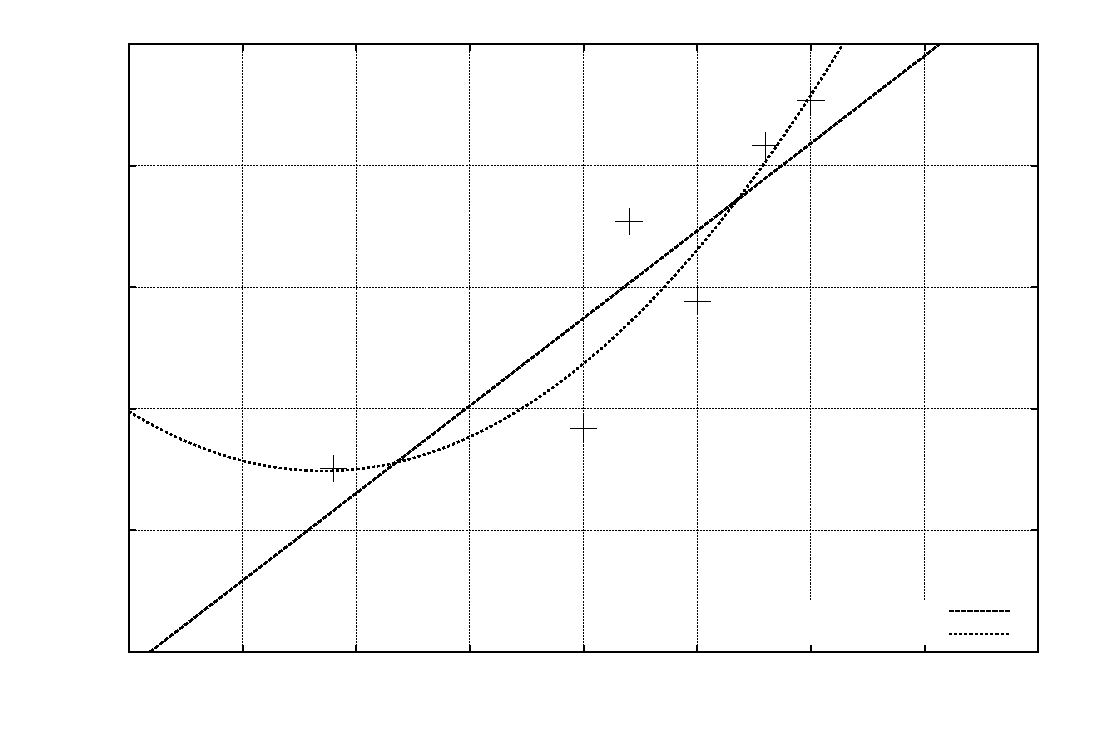
\includegraphics{vytezek}}%
    \gplfronttext
  \end{picture}%
\endgroup

\caption{Závislost výtěžku na protonovém čísle pro přechod K$\upalpha$.}
\label{g:vytezek}
\end{graph}

U radioaktivního vzorku jsme naměřili tři peaky v energiích \SI{30.9}{\keV}, \SI{35.1}{\keV} a \SI{80.9}{\keV}. První dva odpovídají spektrálním čarám Cs. Třetí peak program porovnáním s knihovnou vyhodnotil jako rozpad $^{133}$Ba.